\documentclass[conference]{IEEEtran}
\usepackage{iftex}
\ifPDFTeX
  \usepackage[utf8]{inputenc}
  \usepackage[T1]{fontenc}
\fi
\usepackage{amsmath,amssymb,bm,mathtools}
\usepackage{newtxtext,newtxmath}
\usepackage{booktabs,array,graphicx}
\usepackage{placeins}
\usepackage{tikz,pgfplots}
\usetikzlibrary{arrows.meta,positioning,calc}
\pgfplotsset{compat=1.18}
\usepackage[final]{microtype}
\usepackage{cite}
\usepackage[breaklinks=true,hidelinks]{hyperref}
\usepackage[nameinlink,capitalise,noabbrev]{cleveref}
\interdisplaylinepenalty=2500
\emergencystretch=2em
\allowdisplaybreaks
\raggedbottom
\setcounter{topnumber}{5}
\setcounter{dbltopnumber}{5}
\renewcommand{\topfraction}{0.95}
\renewcommand{\dbltopfraction}{0.95}
\renewcommand{\textfraction}{0.05}
\renewcommand{\floatpagefraction}{0.8}
\renewcommand{\dblfloatpagefraction}{0.8}
\makeatletter
\setlength{\@fptop}{0pt}
\setlength{\@dblfptop}{0pt}
\makeatother
\providecommand{\mathdefault}[1]{#1}
\newcommand{\IncludePGF}[1]{\resizebox{\linewidth}{!}{\input{#1}}}
\newcommand{\vc}[1]{\bm{#1}}
\newcommand{\mt}[1]{\bm{#1}}
\newcommand{\R}{\mathbb R}
\newcommand{\C}{\mathbb C}
\newcommand{\E}{\mathbb E}
\newcommand{\tr}{^{\mathsf T}}
\newcommand{\herm}{^{\mathsf H}}
\newcommand{\sk}[1]{[#1]_\times}
\newcommand{\dd}{\mathrm d}
\DeclareMathOperator{\diag}{diag}
\DeclareMathOperator{\blkdiag}{blkdiag}
\DeclareMathOperator{\Var}{Var}
\DeclareMathOperator{\Rea}{Re}
\DeclareMathOperator{\Ima}{Im}
\DeclareMathOperator{\clip}{clip}
\pdfstringdefDisableCommands{\def\bm#1{#1}\def\vc#1{#1}\def\mt#1{#1}}

\title{Adaptive Shared-Mode CARMA\\
Kalman Filtering for Marine Motion (draft)}
\author{%
  \IEEEauthorblockN{Mikhail S. Grushinskiy}
  \IEEEauthorblockA{Independent Researcher, USA, Fair Lawn\\
  Bareboat Necessities GitHub Project\\
  Email: mgrouch@users.github.com}%
}

\begin{document}
\maketitle

\begin{abstract}
Recovering vessel displacement from an inertial unit requires a model that
separates wave acceleration from gravity, sensor bias and low-frequency
drift. This article presents the 27-state shared-mode continuous-time
autoregressive moving-average (CARMA) filter implemented in ocean-IMU.
A stable CARMA(4,1) displacement spectrum supplies restoring dynamics
for stationary wave-motion estimation, without an integral-displacement
pseudo-measurement. Correlated complex excitation represents the amplitude
and phase relationships of motions produced by common directional waves.
A real cascade realizes this three-axis law with six motion states per
axis; together with three attitude-error and six sensor-bias states it
requires 27 error states. We derive the spectral fit, the reduction from
33 states, frequency and amplitude scaling, discrete process covariance,
sensor updates and covariance transport at parameter changes. We then
describe the independent attitude proxy, spectral-moment period estimator,
noise-aware excitation adaptation, coupling confidence and magnetic startup.
The method estimates translation about a local wave equilibrium. Its
stationary prior regularizes displacement; informative magnetic aiding and
suitable motion remain necessary to distinguish attitude errors from
physical acceleration. Paired vessel-response comparisons, engine-vibration
controls and a low--high--low sea-state transition characterize displacement,
attitude and sensor-bias errors. The implementation is experimental, and neither
universal hull response nor nonlinear adaptive stability is assumed.
\end{abstract}

\begin{IEEEkeywords}
Marine motion, CARMA processes, heave, spectral estimation, quaternion
multiplicative extended Kalman filter, stochastic realization.
\end{IEEEkeywords}

\section{Estimation Objective and Architecture}
\label{sec:objective}
The desired quantities are vessel attitude and the surge, sway and heave
associated with waves. Let $\vc p\in\R^3$ be displacement about a local
equilibrium, $\vc v=\dot{\vc p}$, and $\vc a=\ddot{\vc p}$. A local
north--east--down (NED) frame is used throughout; the displayed heave may
reverse the down-positive sign. This displacement is not geographic
position. Steady translation, current and a permanent displacement offset
cannot be recovered from these sensors by choosing a stronger wave prior.

An accelerometer alone cannot be integrated twice reliably: a constant
acceleration error produces a quadratic position error. The method instead
estimates acceleration and displacement jointly with attitude and sensor
biases. Its wave prior says that displacement has a finite, band-shaped
stationary spectrum. The Kalman update selects a trajectory compatible
with both that prior and the measured specific force.

There are three distinct statistical tasks. A fixed, offline spectral fit
sets the \emph{shape} of the displacement prior. Online measurements set
its \emph{time and amplitude scales}. A slower three-axis estimate sets
the \emph{phase and coherence} of directional coupling. These tasks do not
constitute an online refit of all CARMA coefficients.

\begin{figure*}[!t]
\centering
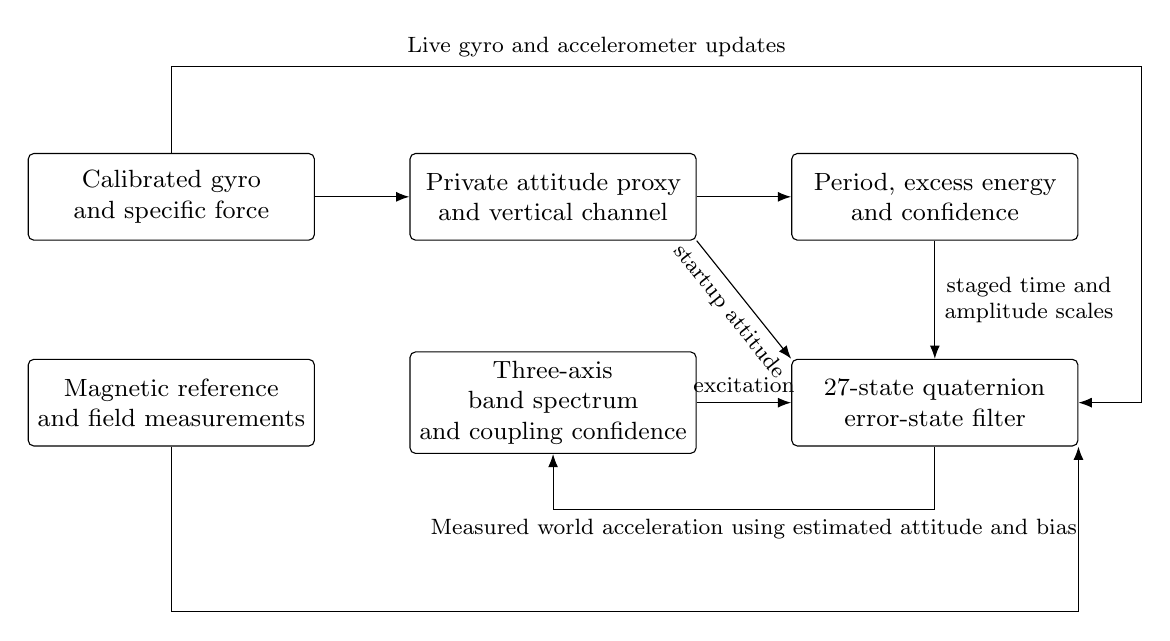
\begin{tikzpicture}[>=Latex, font=\small,
 box/.style={draw,rounded corners=2pt,align=center,minimum height=11mm,text width=34mm},
 lab/.style={font=\footnotesize,align=center}]
 \node[box] (s) {Calibrated gyro\\and specific force};
 \node[box,right=12mm of s] (proxy) {Private attitude proxy\\and vertical channel};
 \node[box,right=12mm of proxy] (tune) {Period, excess energy\\and confidence};
 \node[box,below=15mm of tune] (filter) {27-state quaternion\\error-state filter};
 \node[box,left=12mm of filter] (cross) {Three-axis band spectrum\\and coupling confidence};
 \node[box,left=12mm of cross] (mag) {Magnetic reference\\and field measurements};
 \draw[->] (s) -- (proxy);
 \draw[->] (proxy) -- (tune);
 \draw[->] (tune) -- node[right,lab] {staged time and\\amplitude scales} (filter);
 \draw[->] (cross) -- node[above,lab] {excitation} (filter);
 \draw[->] (filter.south) -- ++(0,-8mm) -| (cross.south);
 \node[lab,below] at ($(filter.south)+(-23mm,-8mm)$) {Measured world acceleration using estimated attitude and bias};
 \draw[->] (mag.south) -- ++(0,-21mm) -| (filter.south east);
 \draw[->] (s.north) -- ++(0,11mm) -| ($(filter.east)+(8mm,0)$) -- (filter.east);
 \node[lab,above] at ($(s.north)+(54mm,11mm)$) {Live gyro and accelerometer updates};
 \draw[->] (proxy.south east) -- node[sloped,below,lab] {startup attitude} (filter.north west);
\end{tikzpicture}
\caption{Information paths. The period and energy branch reads the private
proxy, not the main filter's displacement, attitude or bias. The coupling
branch deliberately uses the main attitude and bias to reconstruct measured
world-frame acceleration. The startup tilt is handed to the main filter;
it is not a continuing attitude measurement in normal operation.}
\label{fig:architecture}
\end{figure*}

\section{Sensors, Tilt and the Need for Magnetic Aiding}
\label{sec:sensors}
Let $\mt R_{wb}$ rotate world vectors into the body frame and
$\mt R_{bw}=\mt R_{wb}\tr$. With $\vc g=g\vc e_z$, the measurement models are
\begin{align}
 \vc\omega_m&=\vc\omega+\vc b_g+\vc n_g,\label{eq:gyro}\\
 \vc f_m&=\mt R_{wb}(\vc a-\vc g)+\vc b_a+\vc n_a,\label{eq:acc}\\
 \vc m_m&=\mt R_{wb}\vc B_w+\vc n_m.\label{eq:mag}
\end{align}
The accelerometer bias can include a configured temperature correction.
Intrinsic calibration and alignment of the three sensors precede these
equations. A known IMU lever arm $\vc r_b$ can also be removed at the wrapper
input by subtracting
$\dot{\vc\omega}\times\vc r_b+
\vc\omega\times(\vc\omega\times\vc r_b)$.
Otherwise the reconstructed translation includes acceleration at the
sensor location.

For a left, body-frame attitude error, the first-order specific-force
perturbation is
\begin{equation}
 \delta\vc f=-\sk{\mt R_{wb}(\vc a-\vc g)}\delta\vc\theta
              +\mt R_{wb}\delta\vc a+\delta\vc b_a.
 \label{eq:ambiguity}
\end{equation}
The same accelerometer residual can therefore be explained by tilt,
translation, or bias. At low motion, a tilt error of $1^\circ$ contributes
about $g\pi/180=0.171$~m/s$^2$ of apparent horizontal acceleration.
A spectral prior makes some explanations less probable; it does not turn
the accelerometer into an independent gravity-direction sensor in waves.

The magnetometer supplies a reference vector that is independent of
translation. Its local attitude Jacobian is
$-\sk{\mt R_{wb}\vc B_w}$, which has rank two for a nonzero field.
Thus magnetic information constrains tilt as well as heading, depending
on field geometry. Rotation about the field remains invisible to one
instantaneous magnetic sample. Gravity information over time, gyro
propagation, motion structure and magnetic corrections must work together.
An unknown or disturbed field, or poor geometry, cannot be repaired simply
by increasing the CARMA order. In this architecture recurrent, informative
magnetic aiding is needed for reliable joint tilt--motion--bias separation;
the presence of magnetometer packets alone does not establish it.

\section{Why a CARMA Displacement Prior?}
\label{sec:carma}
CARMA means continuous-time autoregressive moving-average. Its formal
scalar displacement equation is
\begin{equation}
 P(\mathcal D)p=g_d B(\mathcal D)\dot W,\qquad
 H_\kappa(s)=\frac{B_\kappa(s)}{P_\kappa(s)},
 \label{eq:carma}
\end{equation}
where $\mathcal D=\dd/\dd t$ and $\dot W$ is generalized white noise.
The state-space realization below, rather than differentiation of sampled
noise, defines its implementation. All roots of $P$ are strictly in the
left half-plane. For unit white-noise intensity the two-sided angular
frequency displacement spectrum is
\begin{equation}
 S_p(\omega)=g_d^2|H_\kappa(i\omega)|^2,\qquad
 \Var p=\frac{1}{2\pi}\int_{-\infty}^{\infty}S_p(\omega)\,\dd\omega.
 \label{eq:psd}
\end{equation}
Stable poles give decaying memory and a finite stationary displacement
variance. Complex-conjugate poles represent damped oscillatory response.
The moving-average numerator controls spectral zeros independently of the
restoring poles. A finite-dimensional state model then permits recursive
estimation at irregular sample intervals without storing a long motion
record. These are the relevant reasons to use CARMA here.

\subsection{Why CARMA(4,1)}
The implemented shape is
\begin{align}
 P_\kappa(s)&=L_{1,\kappa}(s)L_{2,\kappa}(s),\nonumber\\
 L_{j,\kappa}(s)&=s^2+2\zeta_j\kappa\omega_j s+(\kappa\omega_j)^2,
 \label{eq:poles}\\
 B_\kappa(s)&=s+\kappa\omega_0,\qquad \omega_0=0.
 \label{eq:zero}
\end{align}
Two damped pole pairs allow a narrow principal response and a broader
roll-off. The first-degree numerator gives relative degree $4-1=3$.
Consequently $S_p=O(|\omega|^{-6})$ at high frequency and the acceleration
spectrum $\omega^4 S_p$ is integrable: ideal acceleration has finite
variance. Acceleration itself is continuous in this realization, whereas
its derivative contains white driving noise. The fitted zero at the
origin gives $S_p=O(\omega^2)$ near DC and strongly discourages very slow
displacement. Four states are sufficient for this scalar spectral shape.

These features motivate the choice; they do not make CARMA(4,1) a unique
or exact law of ocean waves. In particular the ideal JONSWAP surface
spectrum has an $f^{-5}$ tail, so the fit is deliberately over a finite
band. Vessel response and sensor bandwidth also alter the actual motion
spectrum. The retained shape is a compact stochastic prior, not a hull
hydrodynamic model.

\subsection{Why the integral pseudo-measurement is absent}
An acceleration-driven chain with unrestrained velocity and position
integrators has poles at zero. One way to control its drift is to add
$S(t)=\int p(t)\,\dd t$ and repeatedly impose the soft constraint $S=0$.
In the present model, the restoring terms of the Hurwitz polynomial $P$
already make displacement stationary; there are no free position or
velocity integrators in the full state dynamics. The zero in
\cref{eq:zero} further suppresses displacement DC. An extra $S$ state and
an $S=0$ observation are therefore unnecessary for this regularization.

This does \emph{not} assert that the actual displacement is zero or that
an arbitrary initial displacement is observable. The prior chooses the
local wave equilibrium and assigns a distribution about it. It cannot
recover absolute position or eliminate tilt and bias ambiguities. A
covariance regularizer also cannot replace physical magnetic information.
The implementation allocates no $S_x,S_y,S_z$ states and executes no
integral-zero update; shared wrapper settings bearing that name have no
measurement effect in this configuration.

\section{The Offline Spectral Fit}
\label{sec:fit}
The prototype is fitted once to the JONSWAP spectral shape
\cite{jonswap}. Up to an amplitude constant, the target in frequency $f$ is
\begin{align}
 S_J(f)&\propto f^{-5}\exp\!\left[-\frac54(f_p/f)^4\right]
                  \gamma^{r(f)},\nonumber\\
 r(f)&=\exp\!\left[-\frac{(f-f_p)^2}{2\epsilon(f)^2f_p^2}\right],\label{eq:jonswap}\\
 \epsilon(f)&=\begin{cases}0.07,&f\le f_p,\\0.09,&f>f_p.\end{cases}\nonumber
\end{align}
The retained fit uses $f_p=0.29$~Hz, $\gamma=3.3$, and the uniform grid
$f_n=0.17,0.171,\ldots,1.30$~Hz. For trial shape parameters $\vartheta$,
\begin{align}
 d_n(\vartheta)&=10\log_{10}
       \frac{|H_1(i2\pi f_n;\vartheta)|^2}{S_J(f_n)},\nonumber\\
 J(\vartheta)&=\left[\frac1N\sum_{n=1}^N
                 (d_n-\bar d)^2\right]^{1/2}.
 \label{eq:fit}
\end{align}
Subtracting the mean $\bar d$ removes the arbitrary gain: this is a
\emph{shape} fit in decibels. It is not a likelihood fit to live IMU data,
nor a fit of displacement amplitude. The online acceleration statistic
sets the gain separately.

Bounded trust-region least squares uses 48 starts from a fixed random
seed. The constraints are
$f_1\in[0.15,0.60]$~Hz, $f_2\in[0.15,3.00]$~Hz,
$\zeta_1,\zeta_2\in[0.05,1]$, and
$f_0=\omega_0/(2\pi)\in[0,2]$~Hz. The optimum places $f_0$ at its lower
boundary. The stored implementation rounds that value to exactly zero
and uses the coefficients in \cref{tab:shape}.

\begin{table}[!t]
\caption{Prototype shape at frequency scale $\kappa=1$. Frequencies are
pole natural frequencies, not spectral peaks or zero-crossing frequencies.}
\label{tab:shape}\centering
\begin{tabular}{@{}lr@{}}\toprule
Parameter & Implemented value \\\midrule
$f_1=\omega_1/(2\pi)$ & 0.306945 Hz \\
$\zeta_1$ & 0.104191 \\
$f_2=\omega_2/(2\pi)$ & 0.815318 Hz \\
$\zeta_2$ & 0.478188 \\
$f_0=\omega_0/(2\pi)$ & 0 Hz \\\bottomrule
\end{tabular}
\end{table}

The unrounded fit has RMS shape error 1.856~dB on this grid and maximum
absolute residual 17.522~dB. The latter matters: a mean squared log fit
does not guarantee a uniformly small error, especially on the steep
low-frequency shoulder. Its displacement peak is about 0.307~Hz, while its
zero-crossing frequency is about 0.371~Hz. The operating-point adaptation
matches the latter, rather than identifying all three frequencies.

% Analytic curves only: no simulation CSV, external images, or shell escape.
\pgfmathdeclarefunction{carmaunit}{1}{%
 \pgfmathparse{(2*pi*#1)^2/((( (2*pi*0.306945)^2-(2*pi*#1)^2 )^2+(2*0.104191*(2*pi*0.306945)*(2*pi*#1))^2)*(((2*pi*0.815318)^2-(2*pi*#1)^2)^2+(2*0.478188*(2*pi*0.815318)*(2*pi*#1))^2))}}
\pgfmathdeclarefunction{jonswaplog}{1}{%
 \pgfmathparse{10/ln(10)*(-5*ln(#1)-1.25*(0.29/#1)^4+ln(3.3)*exp(-((#1-0.29)/(ifthenelse(#1<=0.29,0.07,0.09)*0.29))^2/2))}}
\begin{figure}[!t]\centering
\begin{tikzpicture}
\begin{axis}[width=\columnwidth,height=47mm,xmode=log,xmin=0.12,xmax=1.5,
 ymin=-65,ymax=3,xlabel={Frequency $f$ [Hz]},ylabel={Peak-normalized PSD [dB]},
 xtick={0.15,0.2,0.3,0.5,1,1.5},xticklabels={0.15,0.2,0.3,0.5,1,1.5},
 grid=major,tick label style={font=\footnotesize},label style={font=\small},
 legend style={font=\footnotesize,draw=none,at={(0.98,0.04)},anchor=south east}]
 \addplot[black,dashed,thick,domain=0.12:1.5,samples=180]
  {jonswaplog(x)-jonswaplog(0.29)};
 \addlegendentry{JONSWAP target}
 \addplot[blue!70!black,thick,domain=0.12:1.5,samples=180]
  {10*ln(carmaunit(x)/carmaunit(0.30736))/ln(10)};
 \addlegendentry{CARMA(4,1) shape}
\end{axis}
\end{tikzpicture}
\caption{The fitted rational spectral shape. Each curve is normalized to
its own peak for display; the fitting objective instead removes the mean
log-level difference over 0.17--1.30~Hz. The rational shape approximates a
finite band and does not reproduce the target's asymptotic tail.}
\label{fig:fit}
\end{figure}

\section{What Is Shared Between the Axes?}
\label{sec:shared}
Directional waves drive several components of vessel motion at once.
For example, horizontal orbital motion and vertical motion can be close
to quadrature: one reaches an extremum near the other's zero crossing.
Hull response adds its own phase. A real covariance between identical
scalar filters captures in-phase or opposite-phase dependence, but cannot
represent that quadrature relationship.

The method shares the \emph{temporal poles and stochastic excitation
structure}, not identical displacement trajectories. Each axis keeps its
own motion state and amplitude. The three driving processes have a
Hermitian covariance $\mt\Sigma=\mt\Sigma_R+i\mt\Sigma_I\succeq0$,
where $\mt\Sigma_R\tr=\mt\Sigma_R$ and
$\mt\Sigma_I\tr=-\mt\Sigma_I$. Real entries describe co-spectral
dependence; imaginary entries describe phase-shifted dependence. An
eigenfactorization of this matrix can be interpreted as a few common
random sources with different complex loadings on the axes. No such
eigenfactorization is required in the sample loop.

To construct the temporal mode, put one root from each pole pair into
\begin{align}
 P_+(s)&=(s-\lambda_{1+})(s-\lambda_{2+}),\nonumber\\
 \lambda_{j+}&=-\zeta_j\kappa\omega_j
         +i\kappa\omega_j\sqrt{1-\zeta_j^2}.
 \label{eq:pplus}
\end{align}
Write $P_+=N_r+iN_i$, with real-coefficient polynomials $N_r,N_i$.
Coefficient conjugation defines $P_-(s)=\overline{P_+(\bar s)}$; hence
$P=P_+P_-=N_r^2+N_i^2$. Choose the real, stable quadratic
$D(s)=s^2+d_1s+d_0$ so that
\begin{equation}
 |D(i\omega)|^2=|N_r(i\omega)|^2+|N_i(i\omega)|^2
 =\frac{|P_+(i\omega)|^2+|P_+(-i\omega)|^2}{2}.
 \label{eq:D}
\end{equation}
Its coefficients and realization are specified in \cref{app:colour}.
For circular complex driving increments $\dd\xi_i=\dd\xi_{r,i}+i\dd\xi_{i,i}$,
define the complex mode
\begin{equation}
 \zeta_i(s)=g_0\frac{B(s)}{P_+(s)D(s)}\xi_i(s),\qquad
 p_i=\Rea\zeta_i.
 \label{eq:complex}
\end{equation}
The increment normalization is
\begin{align}
 \E[\dd\vc\xi\,\dd\vc\xi\herm]&=2\mt\Sigma\,\dd t,\nonumber\\
 \E[\dd\vc\xi\,\dd\vc\xi\tr]&=0.
 \label{eq:circular}
\end{align}
Complex modes are an algebraic representation of real correlated motion;
they do not introduce complex-valued physical positions. Their connection
to multivariate CARMA and sums of complex Ornstein--Uhlenbeck modes is
discussed in \cite{fasen}. The particular factorization here is derived
explicitly rather than assumed from that general representation.

Let $H_c=B/(P_+D)$. The real displacement cross-spectrum is
\begin{equation}
 S_{ij}(\omega)=\frac{g_0^2}{2}
 \left[\Sigma_{ij}|H_c(i\omega)|^2+
       \overline{\Sigma_{ij}}|H_c(-i\omega)|^2\right].
 \label{eq:crossspectrum}
\end{equation}
Using \cref{eq:D}, its diagonal is exactly
$g_0^2\Sigma_{ii}|B/P|^2$. Its imaginary cross-spectrum is proportional to
$\Ima\Sigma_{ij}(|H_c(i\omega)|^2-|H_c(-i\omega)|^2)$ and is odd in
frequency, as required for real motion. Thus sharing preserves the chosen
scalar autospectra while allowing physically useful cross-axis phase.
It also restricts the possible frequency dependence: a single shared shape
and one band-estimated covariance are not a general model of several
independent crossing wave systems.

\section{From 33 States to 27}
\label{sec:reduction}
The complex transfer in \cref{eq:complex} has denominator degree four.
A direct complex state realization has four complex coordinates per
axis, or eight real coordinates. Three such axes plus three attitude
errors, three gyro biases and three accelerometer biases would give
$3\times8+3+3+3=33$ error states.

Only the real output and its derivatives enter the sensors. Rationalizing
the complex denominator yields the \emph{real}, two-input transfer
\begin{equation}
 \begin{aligned}
 p_i(s)&=g_0\frac{B(s)}{P(s)}\eta_i(s),\\
 \eta_i(s)&=\frac{N_r(s)\xi_{r,i}(s)+N_i(s)\xi_{i,i}(s)}{D(s)}.
 \end{aligned}
 \label{eq:realtransfer}
\end{equation}
Both inputs share the real denominator $PD$, of degree six. For the
implemented nondegenerate shape there is no common polynomial cancellation
between that denominator and both numerators. Its minimal real realization
therefore has six states, rather than eight.

The same conclusion follows from observability. In the eight-state
realification each root of $D$ occurs in both the complex mode and its
conjugate. One real displacement output cannot distinguish both directions
in each repeated eigenspace. The corresponding two-dimensional invariant
subspace has identically zero displacement, velocity and acceleration
readout. Removing it eliminates two states per axis, hence six overall.
Rotating the acceleration readout with attitude does not reveal a direction
whose three acceleration outputs are all zero. Magnetic observations act
on attitude, not on those hidden motion directions.

This is a minimal realization of the motion law at fixed parameters. With
compatible projected initial distributions it preserves the complete
three-axis observable Gaussian law, including quadrature spectra and the
corresponding linearized Kalman updates. It is not a universal claim that
arbitrary time-varying coordinates in an unreduced model give the same
adaptive trajectories. Parameter-change transport must be specified; the
actual six-state cascade does so in \cref{sec:commits}.

\subsection{The six-state real cascade}
Set $\bar\omega_j=\kappa\omega_j$,
$u_j=2\zeta_j\bar\omega_j$ and $d=-u_2$ for the implemented zero
$\omega_0=0$. The four scalar spectral states are
$\vc z_i=[p_i,v_i,a_i,\ell_i]\tr$, with
\begin{equation}
 \mt A_4=\begin{bmatrix}
 0&1&0&0\\0&0&1&0\\
 d\bar\omega_1^2&du_1-\bar\omega_1^2&d-u_1&-\bar\omega_2^2\\
 \bar\omega_1^2&u_1&1&0
 \end{bmatrix}.
 \label{eq:A4}
\end{equation}
Its input acts on acceleration through $\vc e_a=[0,0,1,0]\tr$.
The coordinate $\ell_i$ is spectral memory: it is a latent state of the
forcing oscillator in a factored realization. Its equation is
$\dot\ell_i=\bar\omega_1^2p_i+u_1v_i+a_i$.
In particular $\ell_i$ is not an extra $S_i=\int p_i\,\dd t$ state on
which zero is observed.

The two additional states $\vc w_i\in\R^2$ realize the colouring row
\begin{equation}
 \mt V(s)=\frac{[N_r(s)\quad N_i(s)]}{D(s)}
       =[1\quad0]+\mt C_w(s\mt I-\mt A_w)^{-1}\mt B_w.
 \label{eq:V}
\end{equation}
Equation~\eqref{eq:D} implies
$\mt V(i\omega)\mt V(i\omega)\herm=1$. This property, called
\emph{co-inner} or lossless, means that independent unit white inputs give
a unit white output in the stationary Gaussian law. The two states supply
phase structure without changing the single-axis autospectrum.

Use input-normal coordinates, whose unit-input controllability Gramian is
$\mt I_2$:
\begin{equation}
 \mt A_w+\mt A_w\tr=-\mt B_w\mt B_w\tr,\qquad
 \mt C_w=-[1\quad0]\mt B_w\tr.
 \label{eq:inputnormal}
\end{equation}
The final axis state and dynamics are
\begin{align}
 \vc x_i&=[p_i,v_i,a_i,\ell_i,w_{i1},w_{i2}]\tr,\nonumber\\
 \mt A_6&=\begin{bmatrix}\mt A_4&\vc e_a\mt C_w\\0&\mt A_w\end{bmatrix},&
 \mt G_6&=\begin{bmatrix}\vc e_a[1\quad0]\\\mt B_w\end{bmatrix},\label{eq:A6}\\
 \dd\vc x_i&=\mt A_6\vc x_i\,\dd t+
                 g_0\mt G_6\begin{bmatrix}\dd\xi_{r,i}\\\dd\xi_{i,i}\end{bmatrix}.
 \nonumber
\end{align}
There is direct noise only in acceleration and colouring memory;
$\dot p_i=v_i$ and $\dot v_i=a_i$ remain exact kinematic relations.

\begin{table}[!t]
\caption{Error-state allocation. The nominal attitude is carried separately
as a unit quaternion; its four components are not four covariance states.}
\label{tab:states}\centering
\begin{tabular}{@{}llr@{}}\toprule
Block & Coordinates & Count\\\midrule
Attitude error & $\delta\vc\theta$ & 3\\
Gyro bias & $\vc b_g$ & 3\\
North motion & $p_x,v_x,a_x,\ell_x,w_{x1},w_{x2}$ & 6\\
East motion & $p_y,v_y,a_y,\ell_y,w_{y1},w_{y2}$ & 6\\
Down motion & $p_z,v_z,a_z,\ell_z,w_{z1},w_{z2}$ & 6\\
Accelerometer bias & $\vc b_a$ & 3\\\midrule
Total & & 27\\\bottomrule
\end{tabular}
\end{table}

\section{Scaling in Time and Amplitude}
\label{sec:scaling}
Let the unit-gain, unit-scale moments of the four-state shape be
$M_p=\Var_1p$, $M_v=\Var_1v$ and $M_a=\Var_1a$. They are obtained once
in double precision from
\begin{equation}
 \mt A_4(1)\mt P_1+\mt P_1\mt A_4(1)\tr+
                  \vc e_a\vc e_a\tr=0.
 \label{eq:basecov}
\end{equation}
Scaling every pole and zero by $\kappa$ gives
\begin{equation}
 H_\kappa(s)=\kappa^{-3}H_1(s/\kappa).
 \label{eq:similarity}
\end{equation}
Changing integration variable to $\omega/\kappa$ in \cref{eq:psd} yields
\begin{equation}
 \Var p=\frac{g_d^2M_p}{\kappa^5},\qquad
 \Var v=\frac{g_d^2M_v}{\kappa^3},\qquad
 \Var a=\frac{g_d^2M_a}{\kappa}.
 \label{eq:momentscale}
\end{equation}
To request acceleration standard deviation $\sigma_i$, use
\begin{equation}
 g_0^2=\frac{\kappa}{M_a},\qquad \Sigma_{ii}=\sigma_i^2.
 \label{eq:gain}
\end{equation}
Thus $g_d^2=g_0^2\sigma_i^2$ for each marginal, and
\begin{equation}
 \sigma_{p_i}=\frac{\sigma_i}{\kappa^2}\sqrt{M_p/M_a},\qquad
 \sigma_{v_i}=\frac{\sigma_i}{\kappa}\sqrt{M_v/M_a}.
 \label{eq:motionstd}
\end{equation}
At a fixed acceleration scale, doubling the wave frequency quarters the
displacement scale. Doubling $\sigma_i$ doubles displacement and velocity
standard deviations and quadruples all marginal variances.

The prototype displacement zero-crossing frequency is
\begin{equation}
 f_{z,1}=\frac{1}{2\pi}\sqrt{M_v/M_p},\qquad
 \kappa=\frac{f_{\rm op}}{f_{z,1}}.
 \label{eq:kappa}
\end{equation}
This uses the same spectral-moment quantity estimated online. It does not
equate measured period to the reciprocal of a pole natural frequency.
All three axes use the same $\kappa$ and shape. The default amplitudes are
isotropic, $\sigma_x=\sigma_y=\sigma_z$; there is no assumption that their
sample paths are identical.

The colouring realization also scales exactly:
\begin{equation}
 \mt A_w(\kappa)=\kappa\mt A_{w1},\quad
 \mt B_w(\kappa)=\sqrt\kappa\mt B_{w1},\quad
 \mt C_w(\kappa)=\sqrt\kappa\mt C_{w1}.
 \label{eq:colourscale}
\end{equation}
Only the unit-scale two-state factorization is needed. Its input-normal
Gramian remains $\mt I_2$ at every frequency scale.

\section{Discrete Prediction and Sensor Correction}
\label{sec:kalman}
Let $\mt\Pi$ denote the full 27-state estimation covariance, to distinguish
it from the polynomial $P$. For a sample interval $h$, the motion
transition is $\mt F_m=\mt I_3\otimes\mt F_6$ with
\begin{align}
 \mt F_6&=\exp(\mt A_6h),\nonumber\\
 \mt W_R&=g_0^2\mt G_6\mt G_6\tr,&
 \mt W_I&=g_0^2\mt G_6\mt J\mt G_6\tr,\label{eq:WRWI}\\
 \mt J&=\begin{bmatrix}0&-1\\1&0\end{bmatrix}.\nonumber
\end{align}
The real input covariance between axes $i,j$ is
$\Rea\Sigma_{ij}\mt I_2+\Ima\Sigma_{ij}\mt J$ under the normalization
in \cref{eq:circular}. Consequently,
\begin{align}
 \mt Q_R(h)&=\int_0^h e^{\mt A_6t}\mt W_R e^{\mt A_6\tr t}\,\dd t,\nonumber\\
 \mt Q_I(h)&=\int_0^h e^{\mt A_6t}\mt W_I e^{\mt A_6\tr t}\,\dd t,\label{eq:Qpair}\\
 (\mt Q_m)_{ij}&=\Rea\Sigma_{ij}\mt Q_R+
                  \Ima\Sigma_{ij}\mt Q_I.\nonumber
\end{align}
$\mt Q_R$ is symmetric and $\mt Q_I$ is antisymmetric. Since
$\Sigma_{ji}=\overline{\Sigma_{ij}}$, opposite blocks are transposes,
and the complete real $\mt Q_m$ is symmetric positive semidefinite.
$\mt Q_I$ alone is not a noise covariance; it carries the quadrature
part of that complete covariance.

These are exact continuous-to-discrete integrals \cite{vanloan} evaluated
numerically by scaled Taylor series and repeated doubling. For a small
step satisfying $\|\mt A_6h\|_\infty\le1/4$, series terms are accumulated
directly; larger steps use
\begin{equation}
 \mt Q(2h)=\mt Q(h)+\mt F(h)\mt Q(h)\mt F(h)\tr,\quad
 \mt F(2h)=\mt F(h)^2.
 \label{eq:doubling}
\end{equation}
Structural scaling protects small high-order position-noise entries from
loss of relative precision. The code caches a reference discretization and
uses a local step-size series for ordinary timestamp jitter; changes
outside that neighbourhood rebuild the reference. The formula is exact
in continuous time, while the series is truncated to working precision.

The nominal world-to-body quaternion propagates with the measured gyro
minus the estimated gyro bias. With $\vc\omega_c=\vc\omega_m-\hat{\vc b}_g$,
\begin{align}
 \hat q_{wb}^-&=\operatorname{Exp}_q(-\vc\omega_ch)\otimes\hat q_{wb}^+,\nonumber\\
 \mt R_g(t)&=\exp(-\sk{\vc\omega_c}t),\quad
 \mt B_g(t)=\int_0^t\mt R_g(u)\,\dd u,\nonumber\\
 \mt F_{\theta g}&=\begin{bmatrix}\mt R_g(h)&\mt B_g(h)\\0&\mt I_3\end{bmatrix}.
 \label{eq:attitudeprediction}
\end{align}
$\operatorname{Exp}_q$ maps a rotation vector to a unit quaternion.
The positive bias cross-block follows the left world-to-body error
convention used in \cref{eq:ambiguity}. Gyro bias has a random-walk prior.
For gyro-noise and bias-driving intensity matrices $\mt Q_g,\mt Q_{bg}$,
its attitude/bias process covariance blocks are
\begin{align}
 \mt Q_{\theta\theta}&=\int_0^h
 (\mt R_g\mt Q_g\mt R_g\tr+\mt B_g\mt Q_{bg}\mt B_g\tr)\,\dd t,\nonumber\\
 \mt Q_{\theta g}&=\int_0^h\mt B_g(t)\mt Q_{bg}\,\dd t,\quad
 \mt Q_{gg}=h\mt Q_{bg}.
 \label{eq:attitudenoise}
\end{align}
The implementation uses rotation-integral identities and isotropic
shortcuts where available, with Simpson quadrature for the remaining
small matrix integrals.
When enabled, residual accelerometer bias follows a slow OU prior,
$\dd\vc b_a=-\vc b_a\,\dd t/\tau_b+\mt L_b\dd\vc W_b$;
while its startup hold is active both its mean and its own process
covariance are held. When active, $\phi_b=e^{-h/\tau_b}$ and its process
covariance is $\mt L_b\mt L_b\tr\tau_b(1-e^{-2h/\tau_b})/2$.
The attitude, bias and motion blocks retain all
cross-covariances during prediction:
\begin{equation}
 \mt\Pi^- =\mt F\mt\Pi^+\mt F\tr+\mt Q.
 \label{eq:predict}
\end{equation}
The use of repeated six-state dynamics avoids dense 18-state motion
matrix exponentials.

The accelerometer Jacobian has attitude columns from
\cref{eq:ambiguity}, three acceleration selectors rotated by $\mt R_{wb}$,
and accelerometer-bias columns. The magnetometer Jacobian has only direct
attitude columns; its update can still correct motion and biases through
their cross-covariance with attitude. For either observation,
\begin{align}
 \vc r&=\vc y-\hat{\vc y},\nonumber\\
 \mt\Omega&=\mt H\mt\Pi^-\mt H\tr+\mt R_y,\nonumber\\
 \mt K&=\mt\Pi^-\mt H\tr\mt\Omega^{-1},\quad
 \Delta\hat{\vc x}=\mt K\vc r,\label{eq:update}\\
 \mt\Pi^+&=(\mt I-\mt K\mt H)\mt\Pi^-(\mt I-\mt K\mt H)\tr\nonumber\\
           &\quad+\mt K\mt R_y\mt K\tr.\nonumber
\end{align}
Small symmetric systems are solved by factorization, not explicit
inversion. While accelerometer bias is held, its gain rows and the
corresponding update algebra are frozen. The estimated three-vector
attitude correction is injected multiplicatively into the quaternion:
\begin{equation}
 \hat q_{wb}^+=\operatorname{Exp}_q(\delta\hat{\vc\theta})\otimes\hat q_{wb}^-,\quad
 \mt G_\theta=\mt I_3+\tfrac12\sk{\delta\hat{\vc\theta}}.
 \label{eq:reset}
\end{equation}
The attitude-error mean is then set to zero. The covariance is transported
by the full-state congruence with attitude block $\mt G_\theta$, including
every attitude cross-block \cite{markley}. This is the implemented
first-order reset approximation. Bias estimates are projected onto
configured bounds.

The acceleration normalized innovation squared (NIS) is
$\vc r\tr\mt\Omega^{-1}\vc r$. It feeds the coupling monitor described
below. That monitoring should not be confused with per-packet magnetic
outlier rejection: the present core accepts finite nonzero magnetic
observations whose innovation covariance factorization succeeds. Its
diagnostic NIS is not, by itself, a magnetic chi-square gate.

\section{The Independent Proxy and the Wave-Period Estimator}
\label{sec:proxy}
\subsection{Why use a private attitude proxy}
The frontend runs a private gyro--accelerometer complementary observer
of Mahony type \cite{mahony}. It runs from the first sample and produces
up-positive levelled vertical acceleration
\begin{equation}
 a_u=-\vc e_z\tr\mt R_{bw,\mathrm{proxy}}\vc f_m-g.
 \label{eq:verticalproxy}
\end{equation}
Its accelerometer correction corner lies below the wave band; gyro
propagation carries attitude through orbital acceleration. The configured
gain parameters are \texttt{two\_kp}$=0.2$ and
\texttt{two\_ki}$=0.02$. The proportional corner is approximately
0.016~Hz. A fast gravity alignment would follow wave acceleration into a
false tilt. The proxy's yaw is unobservable and may drift; it is removed
when that observer is used as a magnetic accumulation frame.

This branch supplies startup tilt and the default period and energy
measurements. It does not use the main filter's attitude, estimated
acceleration, displacement or bias. Otherwise a main-filter error could
change the apparent sea state, retune its own prior, and reinforce itself.
After startup the proxy continues to supply the tuner; it is not fused as
an additional attitude sensor. The three-axis coupling estimator is a
separate branch and \emph{does} use the main attitude and bias.

\subsection{Period from spectral moments, not acceleration peaks}
For stationary differentiable displacement with moments
$m_0=\Var p$ and $m_2=\Var\dot p$, the spectral zero-crossing period is
\begin{equation}
 T_z=2\pi\sqrt{m_0/m_2}.
 \label{eq:Tz}
\end{equation}
This is generally neither the spectral peak period nor the period of the
acceleration-band carrier. Acceleration weights a displacement spectrum
by $\omega^4$, emphasizing faster components.

The frontend estimates \cref{eq:Tz} with two high-pass stages followed
by two leaky integrations of $a_u$. With leak rate
$\lambda=2\pi(0.02)$~s$^{-1}$, their continuous-time transfer analogues are
\begin{equation}
 \tilde v(s)=\frac{s^2}{(s+\lambda)^3}a_u(s),\qquad
 \tilde p(s)=\frac{s^2}{(s+\lambda)^4}a_u(s).
 \label{eq:periodfilters}
\end{equation}
The actual recursions use timestamp-dependent first-order exponential
coefficients. Bias-corrected exponentially weighted first and second
moments give variances $V_v,V_p$, followed by
\begin{equation}
 T_{z,\mathrm{raw}}=\frac{2\pi}{\sqrt{V_v/V_p-\lambda^2}}.
 \label{eq:Traw}
\end{equation}
The leak subtraction is exact for a narrowband sinusoid in the
continuous-time analogue. For broadband motion it gives a filter-weighted
moment ratio, not an exact unfiltered $T_z$.

The moment horizon is
$\clip(4\hat T_z,20,180)$ seconds. A single canonical log-period state
smooths $\log T_{z,\mathrm{raw}}$ with horizon $0.05\hat T_z$ subject to
implementation guards. Period and frequency are the exponentials of that
state with opposite signs, so they remain exact reciprocals; there is no
second frequency smoother in this chain.

Statistics start after $3/\lambda\simeq23.9$~s to avoid the leaky
integrator startup transient. A usable period requires elapsed time at
least $4/\lambda\simeq31.8$~s and at least one current period of moment
history. This takeover is latched. The stricter settled diagnostic also
requires $6/\lambda\simeq47.7$~s and an accumulated moment weight above
one half. Until usable, the tuner uses a fixed 0.2~Hz prior. These clocks
and energy confidence, rather than the mere existence of a numerical
ratio, determine whether the period can guide adaptation.

\section{Noise-Aware Amplitude and Frequency Adaptation}
\label{sec:adapt}
\subsection{Band energy above the sensor-noise prediction}
The vertical channel is passed through a period-scaled band with
$f_l=0.5 f_t$ and $f_h=4f_t$, limited to 0.01--6~Hz. Its continuous-time
analogue is
\begin{equation}
 H_B(s)=\frac{s b}{(s+a)(s+b)},\qquad a=2\pi f_l,\quad b=2\pi f_h.
 \label{eq:band}
\end{equation}
The band uses the preceding frequency value so the current observation
does not choose its own observation bandwidth. The variance horizon is
approximately four current periods, with bounds and sample-time guards.
Matched exponentially weighted first and second moments give
$V=\E_w[y^2]-(\E_w[y])^2$ after normalization by their accumulated weight.

Configured sensor noise consists of white per-sample standard deviation
$s_n$, bias random-walk intensity $q_b$, and relative uncertainty $u$ in
the predicted noise variance. The no-wave variance is estimated as
\begin{equation}
 V_0=s_n^2G_B+
 \frac{q_b b}{2a(a+b)}-\frac{q_b}{2T_Va^2},
 \label{eq:V0}
\end{equation}
clipped nonnegative. $G_B$ is the band's tracked discrete white-noise
variance gain, and $T_V$ is the variance horizon. The last two terms
approximate the random-walk contribution and removal of its slow mean.
The effective degrees of freedom $\nu$ account for band correlation,
finite horizon and initial accumulated weight; their implemented expression
is given in \cref{app:evidence}.

Define excess variance $E=V-V_0$ and a dimensionless detection statistic
\begin{equation}
 z_E=\frac{E}{V_0\sqrt{2/\nu+u^2}},\qquad
 p_E=\mathcal S\!\left(\frac{z_E-2}{4-2}\right),
 \label{eq:evidence}
\end{equation}
where $\mathcal S(x)=0$ for $x\le0$, $3x^2-2x^3$ for $0<x<1$, and
1 for $x\ge1$. The default evidence-mode excitation target is
\begin{equation}
 \sigma_{\rm target}=c_\sigma\sqrt{p_E\max(E,0)}.
 \label{eq:sigmatarget}
\end{equation}
Although the API calls $p_E$ a probability, it is a configured smooth
evidence weight, not a calibrated Bayesian posterior probability.
No physical wave variance is assigned merely because the sensor has a
noise floor. The numerical acceleration floor, $10^{-5}$~m/s$^2$, exists
only to keep model configuration and floating-point covariance valid.

The evidence branch starts its own band copy at the first acceleration
sample rather than at zero. That avoids interpreting a DC turn-on step as
a minute of wave energy. Its white-noise and bias settings must describe
the installed device. The defaults, $s_n=0.0148$~m/s$^2$ at 200~Hz,
$\sqrt{q_b}=5\times10^{-4}$~m/s$^2/\sqrt{\mathrm s}$ and $u=0.5$, are
simulation settings, not a universal sensor calibration.

\subsection{Rejecting a period unsupported by acceleration energy}
The doubly integrated period proxy emphasizes low-frequency errors.
For small waves, a slow bias or levelling transient can suggest a period
longer than that of the actual acceleration band. An extra low-pass at
$f_h$ forms $y_2$, and a finite-difference derivative forms $\dot y_2$.
After subtracting their modeled no-wave variances, define
\begin{equation}
 f_c=\frac1{2\pi}\sqrt{\frac{V_{\dot y_2}-V_{\dot y_2,0}}
                                  {V_{y_2}-V_{y_2,0}}},\qquad
 r_f=\frac{f_c}{\sqrt{f_lf_h}}.
 \label{eq:fc}
\end{equation}
Only positive excess moments yield a valid ratio. The period confidence is
\begin{equation}
 c_f=\mathcal S\!\left(\frac{z_E-8}{16-8}\right)
         \mathcal S\!\left(\frac{2.5-r_f}{2.5-2.0}\right).
 \label{eq:cf}
\end{equation}
A band centred far below the waves puts its excess energy near the upper
edge, increasing $r_f$ and reducing this confidence. This tests the
frequency support of the period; it is not a new full-spectrum fit.

\subsection{Smoothing and staged activation}
The common scheduling coordinate is $\tau=c_\tau T_z/2$, with default
$c_\tau=1$. Here $\tau$ parameterizes the operating period; it is not an
additional OU acceleration state in the motion model. Frequency and
$\tau$ are clamped to their configured operating envelope. With
$\alpha=1-e^{-h/T_A}$, default $T_A=0.4(T_z/2)=0.2T_z$ subject to guards,
the per-sample candidates obey
\begin{align}
 \tau^+&=\tau+\alpha w_f(\tau_{\rm target}-\tau),\nonumber\\
 \sigma^+&=\sigma+\alpha(\sigma_{\rm target}-\sigma),\label{eq:ema}\\
 w_f&=p_Ec_f\quad\text{once the measured period is usable}.\nonumber
\end{align}
Before takeover, $w_f=1$ follows the fixed period prior. Later, no
supporting wave evidence means $w_f=0$: frequency is held while amplitude
can decay toward the numerical floor. The internal coefficient
$c_\sigma=0.9$ is divided out when assigning acceleration amplitude,
\begin{equation}
 f_{\rm op}=\frac{c_\tau}{2\tau},\qquad
 \sigma_i=c_{\rm gain}\max(10^{-5},\sigma/c_\sigma),
 \label{eq:operatingpoint}
\end{equation}
with $c_{\rm gain}=1$ and equal axes by default.

Every valid IMU sample contributes to the moments and smoothing.
Activation is throttled separately: about every 0.1~s a candidate is
staged, then committed at the start of the next IMU sample. Thus a sample
is predicted and corrected with previously active model parameters.
Changing process coefficients does not reset the posterior to a fresh
stationary covariance on each commit.

\section{Estimating Shared Excitation}
\label{sec:crossestimate}
The coupling branch receives measured world-frame acceleration,
\begin{equation}
 \vc a_{\rm meas}=\hat{\mt R}_{bw}(\vc f_m-\hat{\vc b}_a)+\vc g,
 \label{eq:ameas}
\end{equation}
with temperature and lever-arm corrections when configured. It does not
use estimated CARMA acceleration as its input, but it does depend on the
estimated attitude and bias. Consequently it is not statistically
independent of the main filter.

Complex demodulation at $\dot\phi=2\pi f_{\rm op}$ gives
\begin{equation}
 A_i=\mathcal L\{a_{{\rm meas},i}e^{-i\phi}\},\qquad
 \hat{\mt S}=\E_w[\vc A\vc A\herm].
 \label{eq:demod}
\end{equation}
$\mathcal L$ is two cascaded first-order low-passes with corner
$0.15f_{\rm op}$. The outer-product average has horizon 240~s and is
normalized by accumulated weight. It is Hermitian positive semidefinite
by construction. A practical effective sample count is
$N_{\rm eff}=\max(1,2\min(t,240)\,0.15f_{\rm op})$.
Coupling is not eligible before 120~s of this branch's data.

At an individual frequency, $a_i=-\omega^2p_i$ on all axes, so
$S_{a_i a_z}/S_{a_z a_z}=S_{p_i p_z}/S_{p_zp_z}$.
Within the finite demodulation band this is an approximation when the
response ratios vary with frequency. The estimate describes local
cross-spectral regressions, not a measured full-band hydrodynamic transfer
function.

Partition the band matrix into horizontal and vertical blocks. Its
multiple coherence is estimated as
\begin{equation}
 \gamma^2=\clip\!\left(
 \frac{\hat{\vc S}_{hz}\herm\hat{\mt S}_{hh}^{-1}
                         \hat{\vc S}_{hz}}{\hat S_{zz}},0,1\right).
 \label{eq:coherence}
\end{equation}
If the horizontal block is nearly singular, the implementation uses its
trace-normalized cross-power surrogate instead. Statistical shrinkage is
$s_c=\max(0,1-1/(N_{\rm eff}\gamma^2))$, or zero if coherence is zero.
With coupling confidence $c\in[0,1]$ and user gain $g_c$, set
\begin{equation}
 \vc b=cg_cs_c\frac{\sigma_z^2}{\hat S_{zz}}\hat{\vc S}_{hz},\qquad
 \mt\Sigma=\begin{bmatrix}\mt H&\vc b\\\vc b\herm&\sigma_z^2\end{bmatrix},
 \label{eq:excitation}
\end{equation}
where the default $\mt H=\sigma_h^2\mt I_2$ retains the scheduled
horizontal amplitudes. No measured horizontal autospectrum is promoted
directly to wave energy: horizontal tilt leakage would contaminate it.
The real and imaginary horizontal--vertical terms are retained.
If $q=\vc b\herm\mt H^{-1}\vc b>\rho\sigma_z^2$ ($\rho=0.8$), enlarge
$\mt H$ along the coupling only,
$\mt H\leftarrow\mt H+\frac{\lambda-1}{q}\vc b\vc b\herm$ with
$\lambda=q/(\rho\sigma_z^2)$, so that $\vc b\herm\mt H^{-1}\vc b=\rho\sigma_z^2$;
the measured regression and the cross-wave prior are kept and the
Schur-complement condition guarantees $\mt\Sigma\succeq0$. The study in this
article used the earlier policy, which instead scaled $\vc b$ down to
$q=0.999\sigma_z^2$; that understates the regression under a weak heave RAO
(the TFG companion study compares both). Absent evidence or at zero confidence, the excitation
is diagonal. With isotropic horizontal amplitude this construction
rotates consistently under any change of the north/east heading gauge.

The mapping preserves the measured regression in the \emph{excitation
parameterization}, subject to shrinkage and the positivity cap. It need
not reproduce an arbitrary measured output cross-spectrum exactly:
\cref{eq:crossspectrum} still imposes the shared temporal shape.
Likewise, positivity alone does not ensure that the selected coherence is
physically correct for a particular hull.

\section{Coupling Confidence and Withdrawal}
\label{sec:confidence}
A second demodulation estimate with a 60~s horizon monitors the slower
prior. For each horizontal component form
$\beta_i=\hat S_{iz}/\hat S_{zz}$ with approximate regression variance
\begin{equation}
 v_i=\frac{(1-\gamma_{iz}^2)\hat S_{ii}}{N_{\rm eff}\hat S_{zz}},\qquad
 \gamma_{iz}^2=\frac{|\hat S_{iz}|^2}{\hat S_{ii}\hat S_{zz}}.
 \label{eq:regvar}
\end{equation}
Prior and monitor are compared using
\begin{equation}
 D_\beta^2=\sum_{i=x,y}
 \frac{|\beta_{i,f}-\beta_{i,p}|^2}
 {v_{i,f}+v_{i,p}+0.05^2\max(|\beta_{i,f}|^2,|\beta_{i,p}|^2)+10^{-12}}.
 \label{eq:mismatch}
\end{equation}
The overlapping estimates are correlated; these thresholds are engineering
confidence rules, not a calibrated independent chi-square hypothesis test.
Consistency is withdrawn above 16 and restored below 6.

\begin{table}[!t]
\caption{Additional default gates on shared-mode coupling. These affect
cross-axis excitation; they do not disable the marginal CARMA motion prior.}
\label{tab:gates}\centering\footnotesize
\begin{tabular}{@{}p{.28\columnwidth}p{.66\columnwidth}@{}}\toprule
Evidence & Rule\\\midrule
Warmup & Prior valid after 120~s; short monitor has 60~s history.\\
Band energy & Monitor vertical power divided by its white-noise envelope prediction: zero weight at SNR $\le10$, full at $\ge100$, log interpolation between.\\
Turning & World yaw rate smoothed over 2~s exceeds $3^\circ$/s; withdraw and hold for 30~s.\\
Period change & $|\dd\log f_{\rm op}/\dd t|$ smoothed over 10~s exceeds 0.01/s; withdraw and hold for 30~s.\\
Innovation change & 20~s mean accelerometer NIS exceeds twice its 600~s mean; recover below a ratio of 1.5.\\\bottomrule
\end{tabular}
\end{table}

The envelope noise-power approximation for the SNR gate is
$s_{n,c}^2 h\pi(0.15f_{\rm op})/2$, with separately configured coupling
noise standard deviation $s_{n,c}=0.015$~m/s$^2$. This short-monitor SNR
and the vertical amplitude evidence in \cref{eq:evidence} are different
statistics. The NIS gate uses a ratio because measurement covariance can
be deliberately inflated; an absolute expectation of three is then not
a useful reference for this monitor.

Let $e_c$ be the energy weight when all gates pass, and zero otherwise.
Confidence is smoothed every sample:
\begin{equation}
 c^+=c+(1-e^{-h/T_c})(e_c-c),\qquad
 T_c=\begin{cases}3~\mathrm s,&e_c<c,\\60~\mathrm s,&e_c\ge c.\end{cases}
 \label{eq:confidence}
\end{equation}
The applied gain changes at the approximately 0.1~s confidence cadence
and the excitation is rebuilt at the next step, with or without a model
commit. This
withdraws dependence quickly and restores it slowly. The process tends
toward diagonal excitation smoothly; ordinary smoothing does not snap
$c$ to exactly zero in finite time.

Reducing future process correlation leaves stale posterior motion
cross-covariance. Partition the remaining attitude and bias states as
$r$, horizontal motion as $h$, and vertical motion as $z$. On a confidence
decrease of at least 0.1\% since the last shrink (smaller declines
accumulate) let $\alpha_c=c_{\rm new}/c_{\rm old}$ and use
\begin{align}
 \mt E_{hz}&=\mt\Pi_{hr}\mt\Pi_{rr}^{-1}\mt\Pi_{rz},\nonumber\\
 \mt\Pi_{hz}^+&=\mt E_{hz}+
                \alpha_c(\mt\Pi_{hz}-\mt E_{hz}).
 \label{eq:shrink}
\end{align}
This removes only correlation unexplained by shared attitude and bias
uncertainty. In the conditional motion covariance it is a convex
combination of the current covariance and its horizontal/vertical block
diagonal, so it preserves positivity when the conditioning block is
positive definite. If that factorization fails, the shrink is skipped.
No estimated position, velocity or attitude is changed by this operation.

\section{What Happens at a Parameter Commit?}
\label{sec:commits}
The held physical/spectral coordinates are $[p,v,a,\ell]$. The colouring
coordinates have a stationary scale
$s_i=g_0\sigma_i$. A commit holds their normalized values:
\begin{equation}
 \vc w_i^+=\frac{s_i^+}{s_i^-}\vc w_i^-,\qquad
 \hat{\vc x}^+=\mt M\hat{\vc x}^-,\qquad
 \mt\Pi^+=\mt M\mt\Pi^-\mt M\tr,
 \label{eq:transport}
\end{equation}
where $\mt M$ is identity except for the two colouring entries per axis.
This congruence includes cross-covariances with other axes, attitude and
bias. A frequency change also changes $g_0$ through \cref{eq:gain}, so it
participates in the same scale transport. Coupling-only changes modify
$\mt\Sigma$ without an arbitrary rotation of the motion means.

Input-normal coordinates make the unit colouring Gramian independent of
$\kappa$. With diagonal excitation and the compatible stationary
colouring initialization, the lossless identities in
\cref{eq:inputnormal} preserve a white equivalent scalar drive under this
normalized time/amplitude scheduling. Hence uncoupled marginals retain
the scalar CARMA law during those commits at the linear-model covariance
level for prescribed parameter schedules. This is not a theorem about
closed-loop statistical consistency of the adaptive estimator, nor does
it imply that
arbitrary changing cross-axis excitation has an instantaneous stationary
distribution. The propagated nonstationary covariance remains part of
the estimator state.

\section{Startup and Transition to Live Estimation}
\label{sec:startup}
Starting a joint motion/attitude/bias filter from one acceleration sample
would identify gravity plus wave acceleration as gravity. The frontend
therefore starts first. The main filter is constructed, but the normal
wrapper holds its prediction and correction until handoff. Meanwhile the
proxy integrates gyro and acceleration, the period and energy channels
accumulate data, and magnetic acquisition seeks a reference.

\subsection{Learning a magnetic frame}
Acquisition begins no earlier than 7~s. A gravity-direction quality gate
averages world-frame specific force over 12~s, with a 5~s warmup. It
requires horizontal gravity-direction discrepancy below a sine threshold
of 0.075 for a 2~s hold, and vetoes extreme gyro motion. A separate 30~s
tilt-acquisition fallback can admit a usable reference when that gate
does not settle. This is a startup policy, not a proof of correct tilt.

Magnetometer samples are accumulated in the proxy's \emph{yaw-removed}
tilt frame. An arbitrary drifting proxy yaw must not enter the reference
being learned. At least 128 samples and a 15~s window are required by the
default acquisition configuration. The estimated reference is gauge-fixed
as $\vc B_w=[B_H,0,B_D]\tr$; a one-time yaw rotation puts the learned
magnetic north on $+X$. Its magnitude and inclination are learned, not
assumed known in advance. This north is magnetic north unless declination
is supplied elsewhere.

An initial tilt error can be embedded in that first reference. A second
acquisition starts at 90~s and averages for 30~s in the same independent
proxy tilt frame. It refines the reference after the proxy has had time
to settle. Configured hard-iron estimation is separate from the basic
wave-state model and must satisfy its own excitation and quality checks.

\subsection{Handoff and bias release}
The normal handoff requires an initialized proxy, at least 8~s elapsed,
held gravity agreement, acquired north when magnetic aiding is enabled,
and a ready tuner with a usable measured period. The latter ordinarily
prevents normal handoff before roughly 31.8~s. A 150~s timeout uses the
best available attitude but still requires the aligned gravity branch;
it does not authorize the antipodal tilt. Magnetic acquisition timing can
extend the applicable timeout floor. Thus timeout entry is a degraded
startup path, not evidence that every quality condition was satisfied.

The nominal attitude is seeded from the proxy tilt composed with the
learned yaw gauge. Handoff standard deviations are 0.035~rad for tilt and
0.087~rad for magnetically gauged yaw; without a yaw gauge the latter is
1.5708~rad. The current process scale is applied, and the motion covariance
is seeded from its stationary prior with unrelated cross-blocks cleared.
This initialization is different from the later parameter commits, which
carry the posterior forward.

Accelerometer-bias adaptation remains held at handoff. The default unlock
requires 250 actually accepted magnetic corrections spanning more than
one second, and Live status. A correction counted as accepted by the core
still does not certify strong geometric information or an undisturbed
field. Holding bias initially reduces the chance that it absorbs a
settling tilt error. It does not remove the physical need for subsequent
magnetic service.

The coupling prior and short monitor receive data only once main-filter
accelerometer updates run. Their 120~s and 60~s clocks therefore begin
after handoff in the normal wrapper, not at power-on. With default
confidence initially zero, initial Live estimation has diagonal excitation;
shared coupling is acquired gradually later. An optional presentation
detrender can process output displacement, but is not an $S=0$ update
and is not part of the 27-state estimation model.

\section{Per-Sample Execution}
\label{sec:execution}
The order of operations is part of the adaptive algorithm. During
bootstrap only the measurement frontend and magnetic acquisition run.
In Live operation one IMU sample is processed as follows:
\begin{enumerate}
 \item Apply any staged tune from the preceding sample; refresh motion
 dynamics, paired covariance integrals and colouring-coordinate transport
 when required.
 \item Condition the measured specific force, including a configured
 lever arm, and advance the private attitude proxy. Update the configured
 vibration/low-wave measurement-noise conditioning.
 \item Predict the main quaternion, motion and biases over the actual
 sample interval. Propagate the complete covariance.
 \item Reconstruct measured world acceleration for both cross-spectral
 accumulators. Perform the accelerometer update and multiplicative reset.
 Update coupling confidence using the new innovation diagnostic.
 \item Run the tilt watchdog; advance the vertical acceleration tracker,
 energy statistics and tuner. Stage a tune when the commit clock is due.
 Advance the independent wave-period estimator for subsequent samples.
\end{enumerate}
Magnetic samples arrive on their own clock. They acquire or refine the
reference during startup and deliver vector corrections in Live
operation. Coupling confidence withdrawal can shrink conditional motion
covariance at its own approximately 0.1~s cadence, while the new excitation
is realized on the next motion-model refresh. The acceleration-band
frequency tracker also serves wave-direction reporting; its carrier is
not substituted for the zero-crossing period in \cref{eq:kappa}.

\input{csm-validation.tex-part}

\section{Scope and Limitations}
\label{sec:scope}
The stationary displacement and acceleration marginals, the six-state
realization and the positive-semidefinite excitation are algebraic
properties of the stated model. They are not an end-to-end theorem for
the nonlinear, adaptive, gated, finite-precision filter. Actual vessel
motion can disagree with its fixed spectral shape, default amplitude
ratios, narrowband cross-spectrum or sensor-noise model.

The repository's committed synthetic study uses 26 scenarios and 30
sensor-noise seeds per scenario for this filter. On its spread-JONSWAP
case the mean three-dimensional displacement RMS is 25.4~mm; reducing
the simulated heave response to half gives 32.5~mm. A coloured
accelerometer disturbance of 4~mg with a 2~s time scale gives 817.5~mm.
These are absolute results for the method, from the pinned study bundle,
with scoring beginning at 300~s; they are not sea-trial accuracy claims.
The coloured-noise case is a warning that a disturbance inside the
wave band can pass energy detection and be assigned to motion.

There is a related limitation in coupling normalization. A changed
horizontal-to-vertical hull response can make the prior over-coupled even
when the slow and short measured regressions agree. Their agreement
tests temporal consistency; it does not validate the assumed marginal
amplitude ratio. The positivity cap in \cref{eq:excitation} bounds a
covariance mathematically, not by measured hull coherence. More complex
crossing seas may also need several spectral modes rather than one
operating period.

The dense error covariance contains $27^2=729$ scalar entries, or 2916
bytes in single precision. The full filter object is larger because it
also carries discretization caches, cross-spectral statistics and
confidence state. The implementation uses fixed-size blocks after
construction. The filter remains experimental; its deployment requires
measured noise parameters, valid calibration, suitable magnetic conditions
and validation for the vessel and IMU placement.

\section{Conclusion}
The method combines a stationary CARMA displacement law, shared complex
excitation and quaternion error-state estimation. CARMA(4,1) supplies
damped restoring dynamics, finite acceleration variance and a fitted
low-frequency zero, so an integral-displacement pseudo-observation is not
needed. Sharing represents the phase of motion driven by common waves;
minimal real realization retains that law in six motion states per axis,
giving 27 error states overall. Spectral-moment period and excess
acceleration energy scale the fixed shape, while slower cross-spectral
evidence controls coupling. The private proxy and staged startup provide
a usable initial frame; recurrent magnetic information helps keep
gravity leakage distinguishable from physical wave motion. These roles
are complementary and are all needed to understand the implemented
estimator.

On the declared vessel-response ensemble, the paired comparisons favor the
CARMA displacement priors over OU--III for heave and three-dimensional
error, with a smaller additional contribution from shared excitation.
Machinery vibration nevertheless produces large errors, and the fixed
covariance-inflation gain is not uniformly helpful. The bias and transition
plots expose residual ambiguity and adaptation behavior alongside the
aggregate scores. These findings concern the prescribed hull, corruption
model and tuning settings; they do not establish sea-trial performance.

\FloatBarrier
\appendices
\section{Constructing the Two-State Colouring Filter}
\label{app:colour}
At unit scale write $P_+(s)=s^2+b_1s+b_0$ with complex coefficients.
Then $N_r=s^2+\Rea b_1s+\Rea b_0$ and
$N_i=\Ima b_1s+\Ima b_0$. The even polynomial on the right of
\cref{eq:D} is $\omega^4+\beta\omega^2+\gamma_0$, where
\begin{align}
 \gamma_0&=|b_0|^2,\quad \beta=|b_1|^2-2\Rea b_0,\nonumber\\
 d_0&=\sqrt{\gamma_0},\quad d_1=\sqrt{\beta+2d_0}.
 \label{eq:Dcoeff}
\end{align}
Positive $d_0,d_1$ select the stable real spectral factor. An explicit
observer-form realization of \cref{eq:V} is
\begin{align}
 \mt A_0&=\begin{bmatrix}-d_1&1\\-d_0&0\end{bmatrix},\quad
 \mt C_0=[1\quad0],\nonumber\\
 \mt B_0&=\begin{bmatrix}\Rea b_1-d_1&\Ima b_1\\
                         \Rea b_0-d_0&\Ima b_0\end{bmatrix}.
 \label{eq:observercolour}
\end{align}
Solve $\mt A_0\mt X+\mt X\mt A_0\tr+\mt B_0\mt B_0\tr=0$,
factor $\mt X=\mt L\mt L\tr$, and transform with $\mt L^{-1}$.
An orthogonal two-state rotation then makes $\mt B_w$ upper triangular
with positive diagonal, fixing otherwise arbitrary coordinate freedom.
The result satisfies \cref{eq:inputnormal}. The implementation uses
closed-form two-by-two algebra for this construction, once per shape,
then uses \cref{eq:colourscale} at each frequency scale. A generic
factorization in every sample is unnecessary.

\section{Noise Moments Used by the Evidence Channel}
\label{app:evidence}
Put $c_n=s_n^2h$, $q'=q_b/(ab)$ and let $w$ be the accumulated normalized
EMA weight. The implemented effective degrees of freedom are
\begin{equation}
 \nu=2T_V(a+b)\frac{(c_n+q')^2}
 {c_n^2+2c_nq'+q'^2(a^2+3ab+b^2)/(ab)}\frac{w}{2-w}.
 \label{eq:nu}
\end{equation}
The weight correction accounts for the shorter record immediately after
startup. Under white noise alone the long-record expression reduces to
$2T_V(a+b)$. The extra low-pass and derivative in \cref{eq:fc} use
the continuous-time no-wave moment approximations
\begin{align}
 V_{y_2,0}&=\frac{c_n b^3}{4(a+b)^2}
       +\frac{q_b b(a+2b)}{4a(a+b)^2}-\frac{q_b}{2T_Va^2},\nonumber\\
 V_{\dot y_2,0}&=\frac{c_n b^4(2a+b)}{4(a+b)^2}
                       +\frac{q_b b^3}{4(a+b)^2}.
 \label{eq:noisemoments}
\end{align}
Finite discrete differences, changing band corners and non-white
installation noise limit these approximations. The uncertainty term $u$
in \cref{eq:evidence} prevents treating the nominal noise prediction as
an exact known quantity.

\section{Implementation and Reproducibility}
\label{app:implementation}
The source map in \cref{tab:sources} identifies the default six-state
cascade, sensor-update core, adaptation, and independent frontend.
The equations in this article specify the method without requiring those
files to understand it. The public experimental wrapper is
\path{SeaStateFusion_CarmaSharedModes}.

\begin{table}[!t]
\caption{Source map relative to the repository root.}
\label{tab:sources}\centering\footnotesize
\begin{tabular}{@{}>{\raggedright\arraybackslash}p{.29\columnwidth}>{\raggedright\arraybackslash}p{.65\columnwidth}@{}}\toprule
Part & Source\\\midrule
Spectral shape and fit & \path{tools/carma_fit.py}; \path{src/kalman_carma/CarmaVerticalModel.h}\\
Minimal motion and paired noise & \path{src/kalman_carma_shared_modes/CarmaSharedModesMotion.h}\\
Measurement and reset & \path{src/kalman_carma/Kalman3D_Wave_CARMA3.h}\\
Scale scheduling & \path{src/kalman_carma/SeaStateFusionFilter_CARMA3.h}\\
Wave evidence & \path{src/kalman_carma/CarmaWaveEvidence.h}\\
Cross spectrum & \path{src/kalman_carma/CarmaCrossSpectrumEstimator.h}\\
Coupling confidence & \path{src/kalman_carma_shared_modes/CarmaCouplingConfidence.h}\\
Proxy and handoff & \path{src/kalman_common/MarineWaveFrontEnd.h}; \path{src/kalman_common/ProxyStartupFusion.h}\\\bottomrule
\end{tabular}
\end{table}

The spectral objective can be reproduced by running
\texttt{python3} \path{tools/carma_fit.py}; the retained result is
\path{reports/results/carma_model/carma_fit.json}. The motion and estimator
checks live in \path{tests/kalman_carma_shared_modes/}. The full scenario
driver is \path{tools/carma_shared_modes_study.py}. Absolute numbers in
\cref{sec:scope} come from
\path{reports/results/kalman_carma_shared_modes/}, whose manifest pins
source revision \texttt{08f9900032b5} (full hash in the manifest),
with 30 seeds and a 300~s scoring start. They are existing evidence,
not new runs generated for this explanatory article.

The method's derivations and spectral-fit figure are self-contained.
The comparative and degradation studies are reproduced with
\path{tools/carma_shared_modes_validation.py}. Its \texttt{run} stage reads
the pinned dataset and built simulators; its \texttt{figures} stage rebuilds
the charts and tables from the committed scores and compact drawing traces,
without rerunning the simulations. The ordinary
\path{plots/kalman_carma_shared_modes/draw_plots.sh} pipeline also generates
these figures. From this
directory the complete article builds with two runs of \texttt{lualatex} on
\path{kalman_carma_shared_modes.tex} after that generation step.
Project source and evidence are available
at \url{https://github.com/bareboat-necessities/ocean-imu}.

\section*{Acknowledgments}
ChatGPT assisted with source inspection, mathematical drafting and
editorial preparation under author supervision. The author is responsible
for the method, validation and final manuscript.

\begin{thebibliography}{9}
\bibitem{jonswap}
K. Hasselmann \emph{et al.}, ``Measurements of wind-wave growth and swell
decay during the Joint North Sea Wave Project (JONSWAP),''
\emph{Erg\"anzungsheft zur Deutschen Hydrographischen Zeitschrift},
Reihe A (8), no. 12, 1973.
\bibitem{fasen}
V. Fasen-Hartmann and M. Scholz, ``Factorization and discrete-time
representation of multivariate CARMA processes,'' arXiv:2102.11681, 2021.
\bibitem{vanloan}
C. F. Van Loan, ``Computing integrals involving the matrix exponential,''
\emph{IEEE Trans. Autom. Control}, vol. 23, no. 3, pp. 395--404, 1978.
\bibitem{markley}
F. L. Markley, ``Attitude error representations for Kalman filtering,''
\emph{J. Guid. Control Dyn.}, vol. 26, no. 2, pp. 311--317, 2003.
\bibitem{mahony}
R. Mahony, T. Hamel and J.-M. Pflimlin, ``Nonlinear complementary filters
on the special orthogonal group,'' \emph{IEEE Trans. Autom. Control},
vol. 53, no. 5, pp. 1203--1218, 2008.
\bibitem{tvg-nlo}
T. H. Bryne, T. I. Fossen and T. A. Johansen, ``Nonlinear observer with
time-varying gains for inertial navigation aided by satellite reference
systems in dynamic positioning,'' in \emph{Proc. Mediterranean Conf.
Control and Automation}, 2014, pp. 1353--1360.
\end{thebibliography}
\end{document}
